\begin{chapabstract}
\small{
The main goal of this Ph.D. dissertation is to address the problem of source detection, illustrated by \autoref{s:sag} while overcoming the limitations of the analysis techniques currently being investigated to be applied in the real-time context, described in \autoref{s:gamma-ray-data-analysis}. In addition, since this work is framed in the context of the software development for the \textit{Array Control and Data Acquisition} (ACADA) system, the software requirements described in \autoref{s:sag} have been taken into account. This chapter is organized as follows. 
\autoref{s:anomaly-detection} will describe the proposed anomaly detection technique to address the source detection problem. \autoref{ss:data-pipeline} will describe the data pipeline that has been developed to generate input data. \autoref{ss:p-values} will describe the p-value analysis to associate each positive classification with a gaussian statistical significance. \autoref{s:non-stationary-settings} will investigate several problems that can arise during the telescope observations and how those problems can affect the proposed system. 
}\\
\begin{center}
\noindent\makebox[0.8\linewidth]{\rule{0.66\paperwidth}{0.4pt}}
\end{center}
\vspace{1cm}
\end{chapabstract}
\section{The proposed anomaly detection method}
\label{s:anomaly-detection}
This section will describe the proposed anomaly detection technique. As explained in \autoref{s:anomaly-detection}, the goal of anomaly detection is the identification of rare items, events, or observations which deviate significantly from the majority of the data and do not conform to a well-defined notion of normal behavior.
This work applies anomaly detection analysis to light curves in the gamma-ray energy spectrum. The y-axis represents the \textit{flux} quantity,  describing how much light a source emits. The goal is to identify high-energetic phenomena called \textit{Gamma-Ray Bursts} (GRB), described in \autoref{s:Gamma-Ray-Bursts}. This problem is called \textit{source detection}, and it will be framed into the two  use cases of \textit{serendipitous discoveries} (\autoref{s:serendipitous-discoveries}) and \textit{follow-up observations} (\autoref{s:follow-up-observation}) that require real-time analysis of the data. The problem can be addressed by using an anomaly detection approach considering the \textit{normal data} as the signal coming from a sky region where no sources are present but only background. In contrast, \textit{anomalous data} is defined as the signal coming from a sky region where a source is present (along with background).
The proposed method belongs to the model-based family of techniques to detect multivariate subsequence anomalies described in \autoref{ss:ad-subsequence-multivariate}. It is based on an autoencoder that learns the time series behavior of normal samples. It thereafter uses reconstruction error as anomaly criteria (\autoref{ss:anomaly-criteria}) to detect anomalies. 
Consider a time-series $\bm{X} = \{\bm{x_1}, \bm{x_2}, ..., \bm{x_L}\}$ of length $L$, where each point $\bm{x_i} \in R_3$ is a 3-dimensional vector of flux values. As we will see in \autoref{ss:data-pipeline}, 
the vector of flux values is composed of logarithmically spaced energy bins between 0.04 and 1 TeV. We consider the scenario where multiple  time series are obtained by taking a window of length $L$ over a larger time series. The autoencoder will be trained on normal samples to minimize the reconstruction error of the decoding step. During the training, the network will learn the model of the background. After training, the autoencoder encodes and decodes data samples and outputs an \textit{anomaly score}. GRBs are then detected as noteworthy deviations from this indicator concerning the anomaly score of the normal samples. The anomaly score is computed with a weighted mean-squared error to give more importance to prediction errors in the lower energy ranges that contain most of the signal. Finally, a sample is classified as an anomaly if the anomaly score is greater than a certain threshold $\tau$. To determine the significance of a GRB detection, the anomaly score is mapped to a p-value through a statistical analysis described in \autoref{ss:p-values}. 

\subsection{The data pipeline}
\label{ss:data-pipeline}
This section will describe the input data and the data pipeline that produces it. As described in \autoref{ss:aperture-photometry}, aperture photometry is a method of measuring the flux of electromagnetic radiation emitted by celestial objects, in this case, gamma-ray sources. It is  measured in units of photons per square centimeter per second (photons $cm^{-2} s^{-1}$). The number of photons is computed considering a spatial region called \textit{region of interest} (RoI). A source's spectrum and light curve can be derived from these measurements. 
The spectrum of a gamma-ray source is a plot of the flux as a function of energy. By measuring the spectrum, astronomers can determine the distribution of energies of the photons emitted by the source and learn about the physical processes responsible for their production. On the other hand, a light curve is a plot of the flux as a function of time. It provides information about how the intensity of the radiation changes over time. The data pipeline developed in this work generates multivariate time series representing light curves for three different energy ranges. The final step of the data pipeline extracts multiple sub-sequences by sliding a window over the light curves. 
A semi-supervised data set of background-only samples is generated at the end of the data pipeline. In particular, for each photon list, several multivariate sub-sequences over three channels are computed. Each sub-sequence point is a flux measurement aggregating one or more seconds of the original photon list. Figure [ref] shows some generated samples. The following sections will explain in detail the components of the data pipeline.

\subsubsection{The photons list simulator module}
\label{ss:dl3-simulator}
The data that is needed for the photometry analysis is produced with simulations. This module aims to simulate the data acquisition of a particular sub-array configuration of CTA, considering its instrument's response function. The output of the simulation is a photon list. A photon list represents the high-energy photons detected by the telescope sub-array. It is a list that records the detection timestamp for each detected photon, their reconstructed energy, and the direction of arrival with their corresponding errors. Monte Carlo simulation techniques are commonly used to generate these photon lists, as they allow for incorporating various physical processes. The simulator described in \cite{dipiano2022ctasagsci} has been adopted. This is a python package that wraps \textit{ctools}, an open-source community-developed software  for the scientific analysis of data from imaging atmospheric Cherenkov telescopes (IACTs), developed in the framework of CTA \cite{Knodlseder_2016}. It has been validated on simulated and real data from H.E.S.S., and Fermi \cite{Knodlseder_2019}. 
Simulations performed with \cite{dipiano2022ctasagsci} can be configured using the following parameters: 
\begin{itemize}
    \item number of simulations (trials): this parameter determines the number of simulated photon lists.
    \item simulation duration (tobs): this parameter determines the duration of the observation in seconds.
    \item instrument response function (irf): different types of telescopes and array configurations have different IRFs. The IRF used for running all simulations is called $North\_z40\_5h\_LST$ which models the instrument response function of an LST-1 telescope located in the northern hemisphere site, observing for 5 hours at $40^{\circ}$ zenith angle. This IRF has been chosen to model extra-galactic observations. Simulated galactic plane observations would require both the diffuse emission and known source models that are not available at the time of writing.
    \item minimum energy, maximum energy, and the field-of-view size (emin, emax, roi): these parameters constrain the output of the simulation. The gamma-ray photon will have energy in the range $[EMIN, EMAX]$ (expressed in TeV), and their direction of arrival will be inside the ROI (a circular region whose radius is expressed in degrees).
    \item simulation type (simtype): the simulated photon list will contain background photons by default. This parameter is also used to consider a GRB model (check the following bullet point) and append to the photon list also the simulated GRB event. 
    \item GRB template (runid): as outlined in \autoref{s:Gamma-Ray-Bursts}, the GRBs events are different in terms of duration and luminosity, and the template models the evolutionary process of the event. It is a 3-dimensional grid of fluxes, 70 temporal bins, and 40 energy bins. Hence, the template defines 70 light curves for each energy bin, and for each light curve, it defines 40 spectra. The simulation will integrate the light curve and the spectra within a time-energy interval in the 2D space of a sky map considering the XML spatial model (RA, DEC) of the point-like source.
    \item GRB start (onset): the delay in seconds between the start of the observation and the start of the GRB event.
    \item GRB position (offset): the sky location of the point-like GRB event. It is expressed by adding an offset in degrees to the map's center.
    \item Calibration database (caldb): this database contains CTA's instrument response functions (IRFs), described in \autoref{ss:caldb}. The calibration database used in this work is tagged by version \textit{prod5 v0.1} \cite{zenodo_2021}.
\end{itemize}
To speed up the simulation process, the python code of the simulation script has been rewritten to support batch parallelization with SLURM. The output of the simulations are photons list in FITS format \cite{fitswebsite} that list  each detected photon along with the detection timestamp, their reconstructed energy, and the direction of arrival.

\subsubsection{Integrator module}
\label{ss:integrator-module}
This software module takes as input the photon lists generated by the simulator, along with several other parameters. It integrates the gamma-ray photons along three dimensions: space, time, and energy. For each photon list as input, it generates a multivariate time series of flux values. This software module has been developed from scratch, trying to optimize the speed of the computations as much as possible. 
The public API is represented by the \textit{OnlinePhotometry} class, which accepts the parameters used in the simulation process and the following configuration parameters. The \textit{integration time} (itime) defines the size of the temporal bins used for the time integration of the photon list. For example, with 500 seconds of observation and an integration time of 5 seconds, we obtain $500/5=100$ points representing a time series of photon counts. The \textit{number of energy bins} that is used to compute the energy bins, logarithmically spaced between $tmin=0.04 TeV$ and $tmax=1 TeV$. Considering more than one energy bin, the integration process will output a multivariate time series of photon counts, dividing the photons in each energy bin. In the latter example, the output data shape would equal $(100,3)$. Finally, the \textit{time series length} (tsl) parameter truncates the time series to have \textit{tsl} points. In the latter example, the output shape would be $(0:tsl, 3)$. After defining the temporal end energy integration parameters, the spatial dimension must also be defined. As outlined in \autoref{ss:aperture-photometry}, the spatial region is a circular sky region defined by a center in sky coordinates and a radius expressed in degrees. Only the photons whose arrival direction falls into the circular region are counted. The circle's center is defined by adding an offset in degrees from the pointing. The pointing is read from the header of the fits file. At the same time, the center of the region is computed automatically with a predefined offset added to the on-axis pointing direction. This is accomplished by providing the parameters \textit{regions\_radius} and \textit{max\_offset} to the \textit{integrate} method. The last step is to transform the time series of photon counts into flux values. 
The flux ($ph cm^{-2} s^{-1}$) can be computed with:
\begin{definition} 
\label{def:flux}
[Flux] $\Phi(E)=\frac{dF}{dE}(E)=\frac{dN_\gamma}{dE dA_{eff} dt_{eff}}$
\end{definition}
where $dN_\gamma$ is the number of excess events in $dE$ energy, $A_{eff}$ is the \textit{effective area} in the chosen source region and $t_{eff}$ is the effective observation time. The effective area $A_{eff}(\theta,E_\gamma)$ is the geometric area where photons are collected, multiplied by an efficiency term that depends on the energy of the incoming photons and its angular distance $\theta$ from the optimal on-axis pointing direction. The CTA observatory has a higher effective area in the high-energy range, but it degrades slowly with respect to the pointing-source angle \cite{tampieri2020real}. Since  \autoref{def:flux} normalizes the photon counts for the effective area, taking into account the degradation of the IRF, which increases while moving away from the telescope's pointing, it's possible to extract the photon counts from multiple regions with different offsets from the optimal on-axis pointing direction. Extracting flux measurements from multiple regions in the sky simultaneously significantly boosts the data generation rate and the field-of-view coverage.
The \textit{OnlinePhotometry} class uses the \textit{RegionsConfig} class, whose responsibilities are the computation of the regions' position and their effective area. As stated at the beginning of this section, this software module has been developed to optimize the computations' speed as much as possible. If every photon list has been simulated using the same coordinates concerning the telescope pointing, the effective area can be computed only once and reused for the processing of each photon list. To be more precise, the effective area must be computed for each region and each energy bin. The \textit{OnlinePhotometry} has a \textit{preconfigure\_regions} method that performs this computation. If this method is not called, the \textit{integrate} method will compute the effective area for each photon list.

Another optimization trick is to consider a ring of regions, i.e., all regions that share the same distance from the on-axis pointing. The effective area computation for this group of regions can be done only once since the $\theta$ angle does not change. \autoref{fig:rings} shows an example of multiple ring regions produced by the \textit{RegionsConfig} class. The white region is centered on the source.
\begin{figure}[t]
\centering
\includesvg[width=0.9\linewidth]{figures/method/rings.svg}
\caption{An example of the rings regions produced by the \textit{RegionsConfig} class. The white region is centered on the source.}
\label{fig:rings}
\end{figure}





\subsubsection{Time series extractor module}
\label{ss:extractor}
The last step of the data generation pipeline is to apply a time series extractor module to extract sub-sequences from the time series generated by the previous step. A sub-window of length \textit{tsl} slides over the original time series with a specific \textit{stride}. The number of sub-sequences the method will extract is dependent on the chosen length (i.e., the shorter the length, the higher the number of sub-sequences) and the chosen \textit{stride} (i.e., the shorter the \textit{stride}, the higher the number of sub-sequences). As we will see in \autoref{ss:p-values}, we will need our samples to be statistically independent, meaning no overlapping among the sub-sequences. This can be accomplished by setting the value of the \textit{stride} equal to the \textit{tsl}. In contrast, during inference, we will need to increase the sample rate generation to increase the inference rate, so a \textit{stride} equal to one is preferred. As stated before, a semi-supervised data set of background-only samples is generated at the end of the data pipeline. In particular, for each photon list, several multivariate sub-sequences of length \textit{tsl}, over three channels, are computed. Each sub-sequence point is a flux measurement aggregating $itime$ seconds of the original photon list.

\subsection{P-value analysis}
\label{ss:p-values}
As outlined in \autoref{ss:sag-requirements}, the Science Alert Generation (SAG) system must be able to generate candidate science alerts, meaning that the positive classification produced by the proposed system must be associated with a gaussian $\sigma$ level of statistical significance. A statistical pipeline based on hypothesis testing has been developed to achieve that. This analysis is used to obtain the threshold $\tau$ to classify the samples as anomalies with a certain $\sigma$ level (\cite{Parmiggiani_2021}) or, on the contrary, to associate with each anomaly score a statistical confidence level (of a positive classification). 
\begin{figure}[t]
\centering
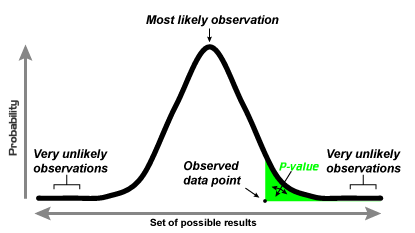
\includegraphics[width=0.6\linewidth]{figures/method/pvalue.png}
\caption{A one-tailed test, showing the p-value as the size of one tail. Credits to \url{https://en.wikipedia.org/wiki/One-_and_two-tailed_tests}}
\label{fig:p-val-one-tailed}
\end{figure}
In hypothesis testing, the initial assumption is that there is no correlation between the predictor and outcome variables in the population. Through statistical tests utilizing data collected, a determination is made as to whether there is enough evidence to reject the null hypothesis in favor of the alternative hypothesis. A two-tailed hypothesis test is designed to show whether the measure is significantly greater than and significantly less than the mean of a population. The two-tailed test gets its name from testing the area under both tails (sides) of a normal distribution. A one-tailed hypothesis test, on the other hand, is set up to show that the measure would be higher or lower than the population mean. \autoref{fig:p-val-one-tailed} illustrates a one-tailed test, showing the p-value as the size of one tail. The level of statistical significance, represented by p-values, serves as the benchmark for these tests. The p-value is the likelihood of obtaining the study results by chance if the null hypothesis is true.
\begin{definition}
\label{def:pvalues} 
The p-value is the inverse of the cumulative distribution function of the test statistic and defines the probability of obtaining a value greater or equal to a threshold $h$ when the null hypothesis is true:
$$ p(ts \geq h) = \int_{h}^{\infty} \phi(x) \,dx $$
where $ts$ is the test statistic of the experiment, $\phi$ is the distribution of the test statistic of the observed experiments, and $h$ is a threshold.
\end{definition}
In other words, the p-value is the likelihood of committing a type I error (false-positive) if one rejects a null hypothesis that is actually true. On the contrary, a type II error (false-negative) occurs if one fails to reject a null hypothesis that is actually false.
The null hypothesis is rejected in favor of the alternative hypothesis if the p-value is less than the established level of statistical significance. 
For example, we can reject the null hypothesis if the p-value is less than $3x10^{-7}$ meaning $> 5\sigma$ confidence in the alternative hypothesis. 
Results with p-values lower than $3x10^{-7}$ can still be false positives every once in $3x10^7$ measures ($\pm$ statistical fluctuations). A metric that considers the number of false positives (or false alarms) per the total number of times the event didn't happen is called \textit{false alarm rate} (FAR). A false alarm rate is also known as the probability of false detection. To not be confused with the false alarm ratio (also abbreviated as FAR), which is the number of false alarms per the total number of warnings or alarms. Regarding hypothesis testing, if P is the probability of committing a type I error (rejecting the null hypothesis when it is actually true) and Q is the probability of making a type II error (failing to reject the null hypothesis when it is actually false), in this study, we prioritize minimizing Q over P to minimize the false positive rate and prevent the system from issuing false science alerts to the scientific community. 

The null hypothesis in this context is represented by the absence of the GRB event in the data. The anomaly score is the test statistic considered in the p-value analysis. To evaluate the p-values, a data set composed of background-only data samples is fed to the autoencoder, and the distribution $\phi$ of the corresponding anomaly scores is computed. Then, the inverse of the cumulative distribution function is evaluated, obtaining a mapping between the test statistics and the p-values. As stated before, a p-value defines the probability of obtaining a value greater or equal to a threshold $h$ when the null hypothesis is true. 
\begin{figure}[t]
    \centering
    \begin{minipage}{0.5\textwidth}
        \centering
        \includesvg[width=\linewidth]{figures/experiments/p_val/model_0_ts.svg}
    \end{minipage}%
    \begin{minipage}{0.5\textwidth}
       \centering
       \includesvg[width=\linewidth]{figures/experiments/p_val/model_0_pvalues.svg}
    \end{minipage}
    \caption{TS distribution and p-values for the autoencoder with convolutional layers in the short-term scenario (integration time = 5 seconds).}
    \label{fig:ts-distribution-and-p-values-cnn-it-5}
\end{figure}
\begin{table}[]
\centering
\begin{tabular}{|crlc|}
\hline
\multicolumn{4}{|c|}{\textbf{p-values}} \\
\hline
threshold & p-value & $\pm$ error &  sigma \\
\midrule
0.003171 &  1.283972e-01 &  1.201785e-04 &  1.134 \\
0.003751 &  6.115264e-02 &  8.293861e-05 &  1.545 \\
0.004476 &  2.277199e-02 &  5.061155e-05 &  2.000 \\
0.005492 &  5.323285e-03 &  2.447028e-05 &  2.554 \\
0.006507 &  1.228234e-03 &  1.175411e-05 &  3.029 \\
0.007667 &  2.312711e-04 &  5.100465e-06 &  3.502 \\
0.009118 &  3.149606e-05 &  1.882250e-06 &  4.001 \\
0.010859 &  3.262092e-06 &  6.057553e-07 &  4.509 \\
0.013760 &  4.499438e-07 &  2.249719e-07 &  4.912 \\
0.013905 &  2.249719e-07 &  1.590791e-07 &  5.047 \\
\bottomrule
\end{tabular}
\caption{An example of p-value analysis for the autoencoder with convolutional layers in the short-term scenario (integration time = 5 seconds). The table shows a subset of all the rows, in particular only the threshold values corresponding to predefined sigma levels are shown.}
\label{tab:p-value-table-cnn-itime-5}
\end{table}
\autoref{fig:ts-distribution-and-p-values-cnn-it-5} and \autoref{tab:p-value-table-cnn-itime-5} show an example of a p-value analysis for the autoencoder with convolutional layer in the short-term scenario (integration time = 5 seconds). More results can be found in \autoref{s:p-values-results} and \autoref{s:appendix-a}. The left panel of the figure shows the test statistic distribution, and the right panel the corresponding p-values. In order to find the corresponding p-value for a given sigma level, first of all we defined the two-tailed probability that we know corresponds to the sigma level of choice. For example, if $sigma=3$, the corresponding two-tailed probability is $p=99.73\%$. The p-value is given by the survival function: $(1-p)=0.0027$. This pvalue describes the probability of having a measure outside the  $\pm3\sigma$. But we want to know which is the one-tailed p-value of that probability since our use cases are constructed on half of a symmetrical distribution. Hence, the previous p-value must be halved obtaining $(1-p)/2=0.00135$. The p-value is then mapped to a threshold value. On the contrary, if we want to know the sigma level of a particular threshold we take the corresponding p-value and find the inverse cumulative distribution function relative to that p-value. Again, since the normal distribution is symmetrical, the absolute value the number of standard deviations rather than  $\pm n\sigma$. if the threshold value is not present in the table, it can be interpolated within the closest two values along with the corresponding p-values interpolation.  

To reach the desired $5\sigma$ level, about $1e^7$ trials need to be simulated and transformed into subsequences fed to the autoencoder to obtain the anomaly scores. Since this process is very computing intensive and has to be repeated several times, each time a new model is deployed in production, the adopted strategy is to generate a data set of about $1e^7$ photon lists with an observation time of 100 seconds. As stated before, the simulation script provided by \cite{dipiano2022ctasagsci} has been rewritten to exploit batch parallelization using Slurm. In addition, a highly parallelizable analysis script has been developed using the same approach to load a trained autoencoder, preprocess the data set, and perform inferences. In particular, each Slurm job takes a batch of photon lists, integrates the photon counts, computes the flux, extracts the time series, scales the data, and performs inference. The time took to process $1e^7$ trials (about $3.5 TB$ of data), using 100 jobs on 60 Intel(R) Xeon(R) Gold 6240 CPU  cores, was about 48 hours. The computational bottleneck was due to the network filesystem that limited the data reading from a SATA hard drive. 

\subsection{Autoencoder architectures}
The architecture of an autoencoder can exploit different types of layers. A convolutional autoencoder typically consists of multiple layers of convolutional and pooling operations. It allows the network to learn spatial hierarchies of features. On the other hand, an autoencoder implemented with recurrent layers is designed to process data sequences, such as text or time series. The autoencoder can learn temporal dependencies and patterns in sequential data with recurrent layers. As mentioned in \autoref{s:ad-with-dl}, more complex and hybrid architectures have been developed such as Temporal Convolutional Networks to  make a CNN layer to understand patterns that occur over a prolonged period \cite{Lea_2016}, ConvLSTM to address the spatio-temporal sequence-forecasting problem \cite{Shi_2015} and transformer (BERT), that implements the current state-of-the-art architectures \cite{Devlin_2018}. In this work, three types of autoencoder architectures have been investigated, based on CNN, RNN, and LSTM layers, resulting in different performance outcomes, both in terms of false positive minimization and training requirements. The architecture has been kept small, with no more than four layers and a few thousand learnable parameters. Since the input data has a low dimensionality, too much complex architecture will be able to memorize and overfit the training data. For the same reason, dropout layers are applied in each model architecture. The dropout layer randomly sets input units to 0 with a certain frequency (20\% in this case) at each step during training time, which helps prevent overfitting. 

\subsection{Autoencoder training}
As stated in \autoref{s:anomaly-detection}, the proposed method belongs to the model-based family of techniques to detect multivariate subsequence anomalies. It is based on an autoencoder trained in a semi-supervised setting to  learn the time series behavior of normal samples. It thereafter uses reconstruction error as anomaly criteria to detect anomalies. A semi-supervised dataset of background-only time series has been generated using the data processing pipeline described in \autoref{ss:data-pipeline}. According to the Science Alert Generation (SAG) design requirements (\autoref{ss:sag-requirements}), the real-time search for transient events should be performed on multiple time scales. The \textit{integration time} setting is used to vary the time scale, integrating the photon counts in tighter or wider time bins. In \cite{tampieri2020real}, and \cite{di2021detection}, the authors explore the capabilities of the Li\&Ma and Full-FoV Maximum Likelihood in the short-term scenario, using very short integration times. The proposed technique is tested under the same extreme setting. In particular, two training datasets have been used, with integration times equal to 5 seconds and 1 second. I will refer to the first data set as \textit{short-term analysis} and to the second data set as \textit{very short-term analysis}. As mentioned in \autoref{ss:integrator-module}, the photon lists can be generated and written to the file system as FITS file only once (unless we want to change the simulation parameters, such as the IRF). Then, using the \textit{OnlinePhotometry} class introduced in \autoref{ss:integrator-module}, several data sets of multivariate time series can be generated. A \textit{DataManager} class has been developed to manage the data used for the autoencoder training and testing. It wraps the \textit{OnlinePhotometry} class to generate the multivariate time series of flux values, extracting the photon counts from multiple regions and applying normalization. This class implements a caching feature to avoid repeating the previous computation multiple times. Finally, it exposes a \textit{get\_train\_set} method to apply all the required data pre-processing to generate training data. In particular, the first step is to extract sub-sequences from the time series. The stride value is equal to 5 to obtain sub-sequences that do not overlap, but shorter strides could be used. The sub-sequences samples are then split into train and validation sets. A MinMax scaler is fitted on the train set and applied to it, scaling the samples to the $[0, 1]$ interval with the formula $ \frac{x-min(x)}{max(x)-min(x)}$. \autoref{tab:training-set-fits} summarizes the simulation parameters to generate the FITS data set, and \autoref{tab:training-set-ts} summarizes the parameters to generate the train set. The resulting samples in the short-term and very short-term settings are respectively 48960 for training, 12240 for validation, and 68000 for training, 17000 for validation. 
\begin{table}[]
\centering
\begin{tabular}{|l|l|}
\hline
\multicolumn{2}{|c|}{\textbf{Simulation parameters}} \\
\hline
trials          & 10                  \\ 
simtype         & bkg                 \\ 
runid           & run0406\_ID000126   \\ 
scalefluxfactor & 1.0                 \\ 
caldb           & prod5-v0.1          \\ 
emin            & 0.04                \\ 
emax            & 1                   \\ 
irf             & North\_z40\_5h\_LST \\ 
offset          & $0.5\degree$                \\ 
roi             & $2.5\degree$                 \\ 
tobs            & 18000               \\ \hline
\end{tabular}
\caption{The parameters used to customize the photon lists simulation for the train set generation.}
\label{tab:training-set-fits}
\end{table}
\begin{table}[]
\centering
\begin{tabular}{|l|l|}
\hline
\multicolumn{2}{|c|}{\textbf{Train test (short-term)}} \\
\hline
integration\_time  & 5 \\ 
number\_of\_energy\_bins & 3 \\ 
tsl & 3600 \\ 
normalize & True \\ 
sub\_window\_size & 5 \\ 
stride & 5 \\ 
validation\_split & 80\% \\ 
Train samples & 48960 \\ 
Validation samples & 12240 \\ \hline
\end{tabular}
\quad
\begin{tabular}{|l|l|}
\hline
\multicolumn{2}{|c|}{\textbf{Train test (very short-term)}} \\
\hline
integration\_time  & 1 \\ 
number\_of\_energy\_bins & 3 \\ 
tsl & 500 \\ 
normalize & True \\ 
sub\_window\_size & 5 \\ 
stride & 5 \\ 
validation\_split & 80\% \\
Train samples & 68000 \\ 
Validation samples & 17000 \\ \hline
\end{tabular}
\caption{The parameters used to configure the \textit{DataManager} class to extract sub-sequences with photometry and to generate the training set. The left panel shows the parameters of the short-term scenario, while the right panel shows the parameters of the very short-term scenario.}
\label{tab:training-set-ts}
\end{table}

The autoencoders have been trained with the \textit{Adam} optimization \cite{Kingma_2014} and a \textit{learning rate} of 0.0001. A 20\% dropout is applied after each layer. As shown by \autoref{tab:training-set-ts}, 80\% of the samples are used for training, while the remaining 20\% is set aside for validation. As already mentioned, the inputs are scaled to the $[0, 1]$ interval. The \textit{batch size} has been set to 32 samples. The autoencoder \textit{loss} (or \textit{anomaly score}) is a \textit{weighted mean squared error} (MSE), defined as the following:
\begin{definition} \label{def:wmse}
[Weighted MSE] $\textbf{WMSE}=\frac{1}{2D}\sum_{i=1}^{D}\bm{w}(\bm{x_i}-\bm{y_i})^2$ where $\bm{w}=[\frac{1}{2}, \frac{1}{3}, \frac{1}{6}]$ and D is equal to the number of points. 
\end{definition}
The reason behind this choice is to give more importance to prediction errors in the lower energy ranges that contain most of the signal. An \textit{early stopping} strategy was considered during training, but the \textit{validation loss} was already flat after five epochs for all models. Hence, the models' weights have been written on disk after five training epochs. \autoref{fig:train-val-loss-itime-5} shows the training and validation losses for the autoencoder with recurrent layers trained in the short-term scenario. More results can be found in \autoref{s:appendix-b}.
\begin{figure}[t]
    \centering
    \begin{minipage}{1\textwidth}
       \centering
        \includesvg[width=\linewidth]{figures/method/training/AnomalyDetector_rnn_l2_u32_train_val_loss_itime_5}
    \end{minipage}
    \caption{An example of train loss and validation loss for the autoencoder with recurrent layers in the short-term scenario (integration time = 5 seconds).}
    \label{fig:train-val-loss-itime-5}
\end{figure}
 


\subsection{Advantages of the proposed method}
This method overcomes the limitations of the analysis techniques described in \autoref{ss:ffov-ml} and \autoref{ss:li-ma}. No assumption on the background model needs to be assumed: the semi-unsupervised learning approach enables the automatic modeling of the background since only background data is used to train the autoencoder. In addition, no hypothesis on the source model needs to be assumed: the anomaly detection approach works by detecting which samples deviate significantly from the normal data. Since there's no need to model the sources, we can overcome the limitation of unrepresentative training data sets. This technique can be applied in a streaming context, identifying outliers in real time as soon as new data points are available. This means that this method can work with overlapping sub-sequences, drastically reducing the time to perform inference. In contrast, the Li\&Ma technique needs to wait for further data since it is limited by the assumption of the statistical independence of the time bins under analysis. Furthermore, using an integration time equal to 1 second, the proposed technique can achieve faster inference, pushing the boundaries of short-term analysis. This is possible because there's no limitation on the minimum amount of signal the method needs to process, overcoming the second limitation of the Li\&Ma technique. Performing real-time analysis of each second of data is also possible because the computational cost of the method is very low due to the autoencoder's simple architecture and the data's size. In addition, multiple models can run in parallel, enabling multi-timescales analysis. According to the expected properties of the signals to detect, the integration time value and the length of the sub-sequences can be chosen accordingly. 


\subsection{How to tackle the problem of non-stationarity of the data}
The background level is not constant and multiple models are trained offline for each IRF (background level).
Concept drift detector to understand when to invalidate the model.

Background changes when: Altitudine/declinazione della sorgente: se si osserva molto basso sull'orizzonte, il segnale (qualunque esso sia) viene degradato molto dell'atmosfera: il segnale attraversa molta più atmosfera rispetto ad un puntamento esattamente a zenith=0 (above head). Le IRF z20 rispetto a alle z60 avranno conteggi del background più bassi, PSF più stretta, area efficace superiore. Anche la luna influenza molto la qualità dell’osservazione, con la luna piena solitamente non si osserva. 
Indeed, in order to perform source detection, the pointing direction of the telescope has a huge impact on the data analysis: if the galactic plane is observed, the diffuse emission, along with all the sources present near the source of interest must be characterized. 
In order to perform source detection, one of the main problems is how to distinguish between the photons that belong to the source of interest to the photons that belong to the galactic or extragalactic background.



\subsection{Non-stationary settings and Online Learning}
\label{s:non-stationary-settings}
During inference the model will process the real-time data generated by the telescopes during an observation. 

In this settings, the stocastic process that generates the data
is not stationary and concept drifts can affect the models' performances. For example, weather changes can degradate the istrument's reponse function and hardware or software malfuctions can arise. In addition, the zenith of the observation changes during time, leading to changes in the background level.  Online learning is a type of machine learning that allows for the analysis and modeling in a streaming fashion, as opposed to batch processing. Concept drift refers to the phenomenon of a dataset's statistical properties changing over time, which can lead to the degradation of the performance of machine learning models trained on such data.
Neural networks are particularly vulnerable to concept drift, as they rely on the assumption that the data distribution remains constant during training and inference. In the presence of concept drift, the model may continue to make predictions based on outdated information, leading to a decrease in accuracy. There are several approaches to address concept drift in online learning for neural networks. One approach is to continuously monitor the performance of the model and detect when a drift has occurred, using techniques such as drift detection methods (DDMs). DDMs can be classified into two categories: instance-based DDMs and feature-based DDMs. Instance-based DDMs monitor the model's error rate on a sliding window of the most recent instances, while feature-based DDMs monitor the distribution of the input features.

We already pointed out that online learning systems, without any explicit change
detection mechanism can adapt to evolving data. The advantage of explicit change
detection is providing information about the dynamics of the process generating data

The model is
updated with the current example. As time goes on, the newly arrived data tend to
erase away the prior patterns. In models, such as artificial neural networks, learning
is inevitably connected with forgetting. The ability to continuously learn from a stream
of examples while preserving previously learned knowledge is known as the stabilityplasticity dilemma [Carpenter et al. 1991a]. It is a dilemma because there needs to be
a balance between being stable to handle noise and being able to learn new patterns.
Some artificial neural networks completely forget the past patterns when exposed to a
new set of patterns; this phenomenon is known as the catastrophic forgetting [French
1994; Polikar et al. 2001].